\documentclass{article}
\usepackage{fullpage}
\usepackage{amsmath}
\usepackage{amssymb}
\usepackage{amsfonts}
\usepackage{stmaryrd}
\usepackage{hyperref}
\usepackage{fixltx2e}
\usepackage{tikz}
\usepackage{tkz-graph}
\usetikzlibrary{shapes,arrows}

\newcommand{\entrynode}[1]{
  \SetVertexNormal[Shape      = circle,
                   FillColor  = black,
                   LineWidth  = 0pt,
                   MinSize    = 0pt]
  \Vertex[L={\tiny\,}]{#1}
  \SetVertexNormal[Shape      = circle,
                   FillColor  = white,
                   LineWidth  = 2pt]
}

\newcommand{\encryptednode}[2]{
  \SetVertexNormal[Shape      = circle,
                   FillColor  = white,
                   LineWidth  = 2pt]
  \tikzstyle{VertexStyle}=[dotted, draw, circle]
  \Vertex[#1]{#2}
  \SetVertexNormal[Shape      = circle,
                   FillColor  = white,
                   LineWidth  = 2pt]
}


\SetUpEdge[lw         = 1.5pt,
           color      = black,
           labelcolor = white,
           labeltext  = red,
           labelstyle = {sloped,draw,text=blue}]

\tikzset{node distance = 2cm}

\title{Anonymity in XIA}
\author{Nicolas Feltman, David Naylor}
\begin{document}
\maketitle

\section{Introduction}
\label{introduction}
The desire for anonymous communication in the Internet has made it a much-discussed issue in both technical and non-technical circles. Users have identified several reasons for wanting online anonymity; in \cite{user-study}, interviews revealed motivations ranging from protecting personal safety to hiding political activity from governments to unknown fears. In one shocking interview from this study, a Romanian woman describes being abducted after posting personal information about herself on a Web site.

Several standard approaches to anonymity have emerged, normally involving some number of explicitly identified proxies (e.g., Tor). Although none of these methods are perfect, they generally meet most users' needs from a technical standpoint. Where many fall short, however, is in making these systems easy to understand and configure for non-technical users; part of our project addresses this issue.

Our goals are three-fold. First, we consider existing methods for achieving anonymous communication in the context of the eXpressive Internet Architecture (XIA)~\cite{xia}. The question we ask ourselves is: Does XIA {\em break} anything? Second, we explore a more interesting question: Does XIA {\em add} anything? As we discuss below, novel features of XIA in many cases allow these existing techniques to be implemented more elegantly and in some cases enable entirely new approaches. Finally, we bring users and developers into the loop. We introduce an extension to the XIA socket API, which provides application developers a dead-easy way to use anonymous communication over XIA. Then, we create a preference pane providing OS level control over the extended API functionality. Anonymization settings are controllable by the user through an intuitive, easily understood GUI.

The rest of this paper is organized as follows: in Section~\ref{background} we introduce pertinent features of XIA and review common terminology related to anonymity from the literature. Section~\ref{approach} examines the use of existing approaches in XIA as well as new ones made possible novel features of the architecture. In Section~\ref{comparison} we compare these approaches to one another in terms of the threats against which they provide protection and we compare the ``current" version of each method to its XIA counterpart. Finally, Section~\ref{implementation} presents our implementation and in Section~\ref{conclusion} we summarize and conclude.


\section{Background}
\label{background}
Before we discuss anonymity in XIA, we will first discuss XIA itself to highlight the features we will make use of later. Then, we will bring some precision to the term ``anonymity" by presenting a review of the terminology used in previous work.

\subsection{Anonymity}
We adopt terminology proposed by Pfitzmann and K\"{o}hntopp~\cite{terminology} to precisely describe various meanings of the term {\em anonymity}:
\begin{description}
\item[Anonymity] The state of not being identifiable within a set of subjects, the {\em anonymity set}.
\item[Unlinkability] Two or more items (e.g., subjects, messages, events, actions, etc.) are no more and no less related than they are related to any other item.
\item[Sender Anonymity] A particular message is not linkable to any sender and no message is linkable to a particular sender.
\item[Recipient Anonymity] A particular message cannot be linked to any recipient and no message is linkable to a particular recipient.
\item[Unobservability] The state of messages being indistinguishable from no messages at all.
\end{description}

\subsection{XIA}
Some features of XIA have implications when it comes to anonymity. We briefly describe the key ideas here and elaborate on their impact on anonymous communication later.
\subsubsection{Principal-Based Communication}
In contrast with today's host-based Internet, XIA provides a framework for communication among \emph{principals}. The idea of principal-based communication is that users should be able to address packets directly to their primary \emph{intent}. For example, a user searching for books on Amazon wishes to communicate with \texttt{www.amazon.com}; he doesn't care which particular Amazon server responds to his request.

In this example, \texttt{www.amazon.com} can be viewed as a \emph{service} principal. In the case where communication with a particular machine truly is the intent, traditional host-based communication can still be achieved via the \emph{host} principal. Other principals include static \emph{content} (e.g., images) and \emph{autonomous domains} (similar to today's autonomous systems).

\subsubsection{DAG-Based Addressing}
Addresses in XIA are represented as DAGs (directed acyclic graphs). Using DAGs allows senders to give the network very detailed instructions about how a packet should be routed. DAGs also allow senders to provide {\em fallback} routes to be used in case the network cannot find the sender's primary intent or does not understand a new principal type. For example, in the scenario above, the user's browser might include the address of a particular Amazon server as a backup in case a packet reaches a router that doesn't know how to find the service \texttt{www.amazon.com} directly. Figure~\ref{fig:proxy-service} depicts a typical DAG.

\begin{figure}
\centering
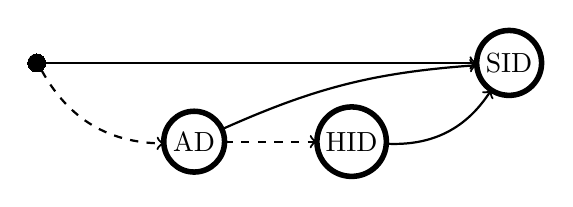
\begin{tikzpicture}
  \entrynode{A}
  \Vertex[x=6,y=0,L=SID]{B}
  \Vertex[x=2,y=-1,L=AD]{C}
  \Vertex[x=4,y=-1,L=HID]{D}
  \tikzstyle{EdgeStyle}=[->]
  \Edge(A)(B)
  \tikzstyle{EdgeStyle}=[dashed, bend right, ->]
  \Edge(A)(C)
  \tikzstyle{EdgeStyle}=[bend left=10, ->]
  \Edge(C)(B)
  \tikzstyle{EdgeStyle}=[dashed, ->]
  \Edge(C)(D)
  \tikzstyle{EdgeStyle}=[bend right, ->]
  \Edge(D)(B)
\end{tikzpicture}
\caption{A typical DAG with two fallbacks. Note that higher edges have higher priority; SID is the primary intent, so the network attempts to route it first. If a router does not know the location of SID, or does not understand services, it uses the first fallback and instead routes the packet to SID's AD. Once in the AD, if a router cannot find SID, the packet is routed to HID, the second fallback, before finally being delivered to the service.}
\label{fig:proxy-service}
\end{figure}


\subsubsection{Intrinsic Security}
All addresses (or, better put, identifiers) in XIA are \emph{intrinsically secure}; exactly what this means varies among principals. For example, a content identifier (CID) is the cryptographic hash of the content itself, enabling anyone receiving the content to verify its integrity. Hosts and services are required to have a public/private key pair; therefore their corresponding identifiers (HIDs and SIDs) are simply the hashes of public keys. A host can sign any communication it generates with its private key and anyone can publicly verify the signature using the host's ID.


\section{Approach}
\label{approach}

\subsection{Proxies}
\label{proxies}
One simple way for a client to achieve anonymity is to route all traffic through a third party, called a ``proxy."  This proxy forwards all communications in both directions, and generally looks indistinguishable from any other client.  In this way, the proxy is the only agent that needs to know the address of the client.  

We consider the example of Amy talking to Betsy using Paul as a proxy.  Betsy alone is unable to link the messages with Amy unless Amy's identity is revealed in the messages themselves.  Similarly, an attacker listening to the communication between Paul and Betsy would be unable to infer Amy's identity.  Alternatively, an attaker listening to the communication between Amy and Paul might be able to link those messages with Betsy, since Betsy's address must be communicated from Amy to Paul at some point.  This can easily be thwarted by encryption of Betsy's address.  An attacker listening to both of Paul's communications (or Paul himself) might be able to link those communications to each other by comparing content or timing.  This can be made very difficult by using several layers of proxies and encryption, such that the chance that all of them are compromised becomes low (\cite{onion}).

To promote maximum orthogonality of features, we decided to describe and implement proxies as an {\em in-network service}, by specifying the desire to send traffic through the proxy in the address DAG of the original packet, rather than encapsulating the packet inside another one addressed only to the proxy.  For instance, the following DAG discribes communication with the end host at SID\textsubscript{E} via the proxy at SID\textsubscript{P}, with proper fallbacks for both.  We go into more detail on the manipulation of these DAGs in \S\ref{proxy}
\begin{center}
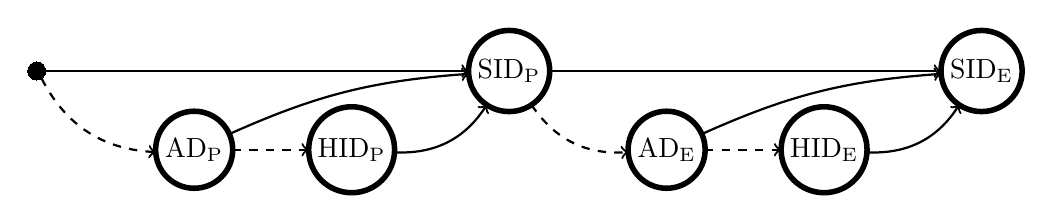
\begin{tikzpicture}
  \entrynode{A}
  \Vertex[x=6,y=0,L=SID\textsubscript{P}]{B}
  \Vertex[x=2,y=-1,L=AD\textsubscript{P}]{C}
  \Vertex[x=4,y=-1,L=HID\textsubscript{P}]{D}
  \Vertex[x=12,y=0,L=SID\textsubscript{E}]{E}
  \Vertex[x=8,y=-1,L=AD\textsubscript{E}]{F}
  \Vertex[x=10,y=-1,L=HID\textsubscript{E}]{G}
  \tikzstyle{EdgeStyle}=[->]
  \Edge(A)(B)
  \tikzstyle{EdgeStyle}=[dashed, bend right, ->]
  \Edge(A)(C)
  \tikzstyle{EdgeStyle}=[bend left=10, ->]
  \Edge(C)(B)
  \tikzstyle{EdgeStyle}=[dashed, ->]
  \Edge(C)(D)
  \tikzstyle{EdgeStyle}=[bend right, ->]
  \Edge(D)(B)
  \tikzstyle{EdgeStyle}=[->]
  \Edge(B)(E)
  \tikzstyle{EdgeStyle}=[dashed, bend right, ->]
  \Edge(B)(F)
  \tikzstyle{EdgeStyle}=[bend left=10, ->]
  \Edge(F)(E)
  \tikzstyle{EdgeStyle}=[dashed, ->]
  \Edge(F)(G)
  \tikzstyle{EdgeStyle}=[bend right, ->]
  \Edge(G)(E)
\end{tikzpicture}
\end{center}

\subsection{Temporary Source Addresses}
\label{temp-ids}
A conceptually simpler approach to achieving anonymity is to use a temporary source address that is unsinkable to you. In today's IP Internet there isn't really a good way to do this. If IP addresses are statically assigned, periodically changing your address is a hassle and may require the involvement of your network administrator, who is unlikely to be willing to assign you a new address every time you want a new identity. Even if addresses are assigned dynamically and you obtain a new one from a DHCP server as often as you'd like, this solution still has major drawbacks. First, most users won't be able to do this from home. A user with a typical home Wi-Fi network can change his computer's IP address to his heart's content, but as his packets pass through his router's NAT, the source address will be overwritten with the public IP assigned to him by his ISP. Further limiting the utility of this approach, your IP address is the source of all traffic you send from your machine, regardless of the application; in some cases, you might want messages from one application to be unlinkable to messages sent by another.

Fortunately, XIA makes the use of temporary source addresses much more feasible. First, consider what normally happens when an XIA application initiates communication with some remote entity. When a host first connects to the network, it contacts a DHCP-like server in its local AD and registers its host ID. Then, when the application opens a socket the operating system will assign the socket an ephemeral service ID (akin to ephemeral ports today). Any packets sent through this socket are given a source address formed form the combination of the host's HID and this ephemeral SID:
\begin{center}
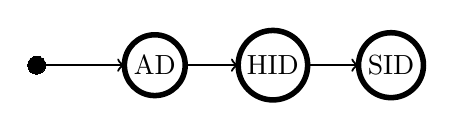
\begin{tikzpicture}
  \entrynode{A}
  \Vertex[x=1.5,y=0,L=AD]{B}
  \Vertex[x=3,y=0,L=HID]{C}
  \Vertex[x=4.5,y=0,L=SID]{D}
  \tikzstyle{EdgeStyle}=[->]
  \Edge(A)(B)
  \tikzstyle{EdgeStyle}=[->]
  \Edge(B)(C)
  \tikzstyle{EdgeStyle}=[->]
  \Edge(C)(D)
\end{tikzpicture}
\end{center}
Now, suppose we want to use a temporary source address to achieve anonymity. Upon creating the socket, the operating system generates an ephemeral SID, as before, only now it takes the additional step of registering it with the local AD as if it were another host ID via the same mechanism it used to register its actual HID when the machine joined the network. Now packets can be sent with this source address:
\begin{center}
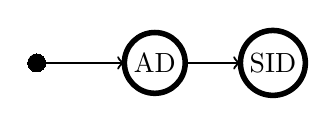
\begin{tikzpicture}
  \entrynode{A}
  \Vertex[x=1.5,y=0,L=AD]{B}
  \Vertex[x=3,y=0,L=SID]{C}
  \tikzstyle{EdgeStyle}=[->]
  \Edge(A)(B)
  \tikzstyle{EdgeStyle}=[->]
  \Edge(B)(C)
\end{tikzpicture}
\end{center}
Note that we have overcome all of the limitations of the temporary address approach in IP: first, since the operating system can simply generate a new public/private key pair and use it to derive a new SID, there is no need to manually obtain a valid available IP address. Second, as XIA uses 160 bit addresses and is in no danger of running out, there will presumably be no need for NATs, so there is no concern that a router will rewrite our temporary source address and compromise our anonymity. Finally, we no longer have the coarse granularity problem temporary IP addresses posed; each {\em socket} gets its own temporary address.

Of course, this strategy is not entirely without limitations. Clearly, anyone using this technique must trust his or her local AD not to reveal the mapping between machine and temporary ID; this may not always be reasonable. On the other hand, this can be looked at as a feature rather than a bug. If an AD maintains a log the SIDs registered with it, law enforcement agencies could potentially access them with a subpoena if criminal activity is suspected. Another limitation, but one that is probably reasonable in most cases, is that traffic anonymized in this manner is not entirely anonymous, but rather linked to you at the AD level. Note that the situation is no better in IP: a temporary IP address still identifies you at the level of your subnet.


\subsection{Principal-Based Traffic Control}
\label{principal-filtering}
A novel approach possible only in XIA is principal-based traffic control. Broadly speaking, a user may to prevent applications from sending packets that are addressed using certain principal types, as the use of a particular principal reveals something about the communication.

For instance, the presence of a CID makes it clear that a packet's purpose is to retrieve a piece of content. Furthermore, it is conceivable that someone might implement a ``reverse lookup" service that does the opposite of the naming service: translates XIDs back into human-readable names. Thus, anyone sniffing our privacy-seeking users's traffic who sees a content request can find out the name of the content from the CID.

Additionally, as new principal types are added to the network in the future, they may similarly reveal information users would prefer to keep private.

In the current XIA design, the operating system would simply drop any packets making use of a disallowed principal (and optionally alert the user). But if a mechanism for partial DAG encryption were adopted, as discussed in \S\ref{in-network-services}, the system could rewrite DAGs in a way that conceals the use of a particular principal. For example, consider a content request with the following DAG:
\begin{center}
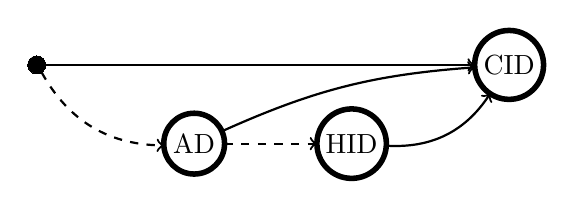
\begin{tikzpicture}
  \entrynode{A}
  \Vertex[x=6,y=0,L=CID]{B}
  \Vertex[x=2,y=-1,L=AD]{C}
  \Vertex[x=4,y=-1,L=HID]{D}
  \tikzstyle{EdgeStyle}=[->]
  \Edge(A)(B)
  \tikzstyle{EdgeStyle}=[dashed, bend right, ->]
  \Edge(A)(C)
  \tikzstyle{EdgeStyle}=[bend left=10, ->]
  \Edge(C)(B)
  \tikzstyle{EdgeStyle}=[dashed, ->]
  \Edge(C)(D)
  \tikzstyle{EdgeStyle}=[bend right, ->]
  \Edge(D)(B)
\end{tikzpicture}
\end{center}
Rather than dropping this packet, the DAG could instead be rewritten as follows, where the dotted line indicates that the CID node is encrypted (with host HID's public key):
\begin{center}
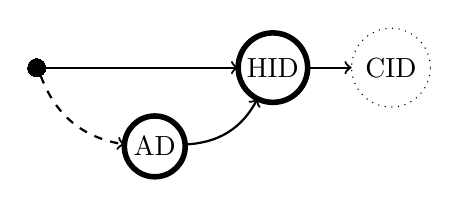
\begin{tikzpicture}
  \entrynode{A}
  \Vertex[x=1.5,y=-1,L=AD]{B}
  \Vertex[x=3,y=0,L=HID]{C}
  \encryptednode{x=4.5,y=0,L=CID}{D}
  \tikzstyle{EdgeStyle}=[->]
  \Edge(A)(C)
  \tikzstyle{EdgeStyle}=[dashed, bend right, ->]
  \Edge(A)(B)
  \tikzstyle{EdgeStyle}=[bend right, ->]
  \Edge(B)(C)
  \tikzstyle{EdgeStyle}=[->]
  \Edge(C)(D)
\end{tikzpicture}
\end{center}



\section{Comparison}
\label{comparison}
Before describing our implementation, we will take a moment to draw comparisons among the approaches described above in terms of the threats against which they protect, as well as compare each method to itself in terms of its implementation and utility in today's IP Internet and XIA... SAY MORE HERE?

\subsection{Approaches vs. Threats}
\begin{center}
	\begin{tabular}{p{2cm} || p{2.5cm} | p{2.5cm} | p{2.5cm} | p{2.5cm} | p{2.5cm}}
	& \textbf{Other Party (e.g., a company)} &	\textbf{Small 3rd Party (e.g., identity thieves)} & \textbf{Large 3rd party (e.g., a government)} & \textbf{ISP} & \textbf{Facebook Friends}\\
	\hline
	\hline
	{\bf Proxy-based service} (e.g., Tor)&&&&\\
	\hline
	{\bf Temporary source ID} &&&&\\
	\hline
	{\bf Principal type filtering} &&&&\\
	\hline
	{\bf Real life pseudonym} &&&&\\
	\hline
	\end{tabular}
\end{center}


\subsection{XIA vs. IP}
\begin{center}
	\begin{tabular}{p{3cm} || p{4.5cm} | p{4.5cm}}
	& \textbf{XIA} 	&	\textbf{IP}\\
	\hline
	\hline
	{\bf Proxy-based service} (e.g., Tor) & Elegantly implemented with DAGs (\S\ref{proxies}) & Packets for final destination are encapsulated in packets to the proxy\\
	\hline
	{\bf Temporary source ID} & Generate new SID and register with local AD via HID registration mechanism (\S\ref{temp-ids}) & Request to be assigned a new IP address from DHCP server or network administrator\\
	& & \\
	& Per-socket granularity & Per-host granularity\\
	\hline
	{\bf Principal type filtering} & Fine grained traffic control (\S\ref{principal-filtering})& N/A \\
	\hline
	\end{tabular}
\end{center}


\section{Implementation}
\label{implementation}
We designed a simple proxy service for anonymizing XIA traffic which we refer to as Envoy. Due to limitations of the underlying XIA codebase, we have implemented only a functional equivalent of Envoy which runs on a single machine and does not handle multiple connections at once. Our version of Envoy is written in Python and communicates over XIA using the Xsocket interface. In \S\ref{proxy} we describe in detail how we use DAGs to route traffic through Envoy. The process of implementing this service brought to our attention a handful of issues relating to in-network services, which we discuss in \S\ref{in-network-services}.

In keeping with our goal to bring users and developers into the loop, we also implemented an extension to the Xsocket API aimed at giving application developers easy access to anonymization tools (\S\ref{api}) and a preference pane enabling users to have the final say as to what applications can and cannot do with respect to anonymity (\S\ref{control}).

\subsection{Single Proxy DAG Manipulation}
\label{proxy}
This version of the protocol assumes that direct communication or authentication between the client and Envoy happens through some other channel.  The client begins by obtaining DAGs for the Envoy service and for the end service.  We will refer to the public addresses of Envoy and the end service as SID\textsubscript{P} and SID\textsubscript{E}. Let the client application be running on a host HID\textsubscript{C} with an ephemeral service identifier SID\textsubscript{A} (for demultiplexing).  It sends the initial packet with the following destination and source addresses (fallback paths omitted):

\begin{center}
    \begin{tabular}{ | l | l |} \hline
    	Dst & Src \\ 
	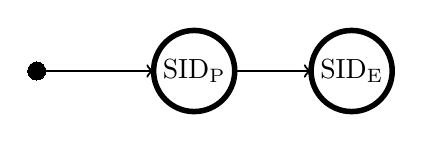
\begin{tikzpicture}
	\entrynode{A}
	\Vertex[x=2,y=0,L=SID\textsubscript{P}]{P}
	\Vertex[x=4,y=0,L=SID\textsubscript{E}]{E}
	\tikzstyle{EdgeStyle}=[->]
	\Edge(A)(P)
	\tikzstyle{EdgeStyle}=[->]
	\Edge(P)(E)
	\end{tikzpicture} &
	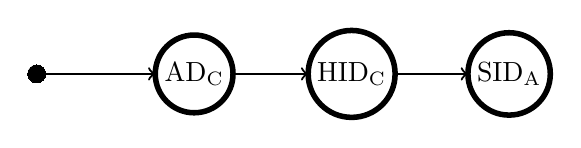
\begin{tikzpicture}
	\entrynode{B}
	\Vertex[x=2,y=0,L=AD\textsubscript{C}]{A}
	\Vertex[x=4,y=0,L=HID\textsubscript{C}]{H}
	\Vertex[x=6,y=0,L=SID\textsubscript{A}]{S}
	\tikzstyle{EdgeStyle}=[->]
	\Edge(B)(A)
	\tikzstyle{EdgeStyle}=[->]
	\Edge(A)(H)
	\tikzstyle{EdgeStyle}=[->]
	\Edge(H)(S)
	\end{tikzpicture}
    \\ \hline
    \end{tabular}
\end{center}

Upon receiving this initial packet, Envoy routes it to a particular machine, henceforth HID\textsubscript{P}, to handle this connection. Since this is the first packet from AD\textsubscript{C}:HID\textsubscript{C}:SID\textsubscript{A}, Envoy creates a new ephemeral service ID, SID\textsubscript{T} and adds this pair to a local table. (Responses from the end service, SID\textsubscript{E}, are sent to Envoy at SID\textsubscript{T}, which looks up the client address corresponding to SID\textsubscript{T} in it's table and forwards the response to the appropriate address.) The machine then forwards the initial packet with the following destination and source addresses:

\begin{center}
    \begin{tabular}{ | l | l |} \hline
    	Dst & Src \\ 
	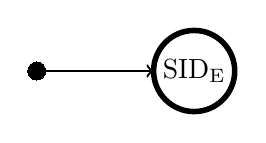
\begin{tikzpicture}
	\entrynode{A}
	\Vertex[x=2,y=0,L=SID\textsubscript{E}]{E}
	\tikzstyle{EdgeStyle}=[->]
	\Edge(A)(E)
	\end{tikzpicture} &
	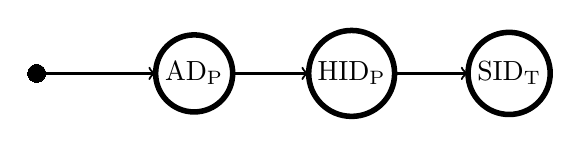
\begin{tikzpicture}
	\entrynode{B}
	\Vertex[x=2,y=0,L=AD\textsubscript{P}]{A}
	\Vertex[x=4,y=0,L=HID\textsubscript{P}]{H}
	\Vertex[x=6,y=0,L=SID\textsubscript{T}]{S}
	\tikzstyle{EdgeStyle}=[->]
	\Edge(B)(A)
	\tikzstyle{EdgeStyle}=[->]
	\Edge(A)(H)
	\tikzstyle{EdgeStyle}=[->]
	\Edge(H)(S)
	\end{tikzpicture}
    \\ \hline
    \end{tabular}
\end{center}

The end service is not aware that it is being communicated with via a proxy. It chooses a machine, HID\textsubscript{E}, to handle this connection, and responds with the following source and destination addresses:

\begin{center}
    \begin{tabular}{ | l | l |} \hline
    	Dst & Src \\
	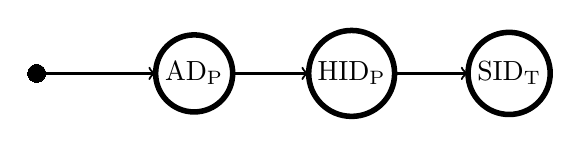
\begin{tikzpicture}
	\entrynode{B}
	\Vertex[x=2,y=0,L=AD\textsubscript{P}]{A}
	\Vertex[x=4,y=0,L=HID\textsubscript{P}]{H}
	\Vertex[x=6,y=0,L=SID\textsubscript{T}]{S}
	\tikzstyle{EdgeStyle}=[->]
	\Edge(B)(A)
	\tikzstyle{EdgeStyle}=[->]
	\Edge(A)(H)
	\tikzstyle{EdgeStyle}=[->]
	\Edge(H)(S)
	\end{tikzpicture} &
	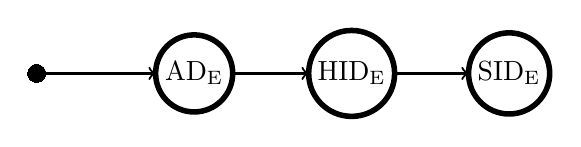
\begin{tikzpicture}
	\entrynode{B}
	\Vertex[x=2,y=0,L=AD\textsubscript{E}]{A}
	\Vertex[x=4,y=0,L=HID\textsubscript{E}]{H}
	\Vertex[x=6,y=0,L=SID\textsubscript{E}]{S}
	\tikzstyle{EdgeStyle}=[->]
	\Edge(B)(A)
	\tikzstyle{EdgeStyle}=[->]
	\Edge(A)(H)
	\tikzstyle{EdgeStyle}=[->]
	\Edge(H)(S)
	\end{tikzpicture}
    \\ \hline
    \end{tabular}
\end{center}

Envoy, in the interest of keeping minimal state, does not remember this bound source address but instead simply sends it back to the client who is responsible for including HID\textsubscript{E} in future packets.

\begin{center}
    \begin{tabular}{ | l |} \hline
    	Dst \\ 
	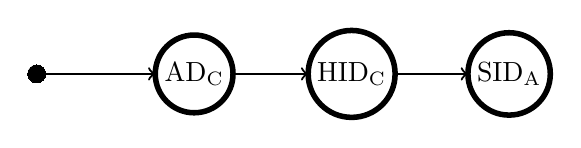
\begin{tikzpicture}
	\entrynode{B}
	\Vertex[x=2,y=0,L=AD\textsubscript{C}]{A}
	\Vertex[x=4,y=0,L=HID\textsubscript{C}]{H}
	\Vertex[x=6,y=0,L=SID\textsubscript{A}]{S}
	\tikzstyle{EdgeStyle}=[->]
	\Edge(B)(A)
	\tikzstyle{EdgeStyle}=[->]
	\Edge(A)(H)
	\tikzstyle{EdgeStyle}=[->]
	\Edge(H)(S)
	\end{tikzpicture} \\ \hline
	Src \\ 
	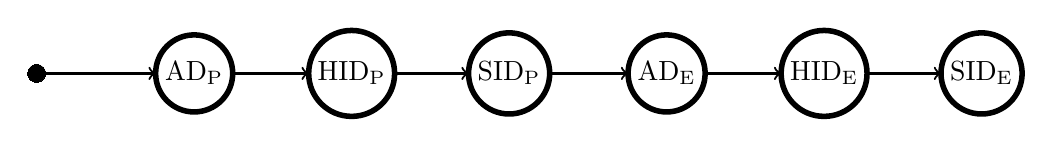
\begin{tikzpicture}
	\entrynode{B}
	\Vertex[x=2,y=0,L=AD\textsubscript{P}]{A}
	\Vertex[x=4,y=0,L=HID\textsubscript{P}]{H}
	\Vertex[x=6,y=0,L=SID\textsubscript{P}]{S}
	\Vertex[x=8,y=0,L=AD\textsubscript{E}]{A2}
	\Vertex[x=10,y=0,L=HID\textsubscript{E}]{H2}
	\Vertex[x=12,y=0,L=SID\textsubscript{E}]{S2}
	\tikzstyle{EdgeStyle}=[->]
	\Edge(B)(A)
	\tikzstyle{EdgeStyle}=[->]
	\Edge(A)(H)
	\tikzstyle{EdgeStyle}=[->]
	\Edge(H)(S)
	\tikzstyle{EdgeStyle}=[->]
	\Edge(S)(A2)
	\tikzstyle{EdgeStyle}=[->]
	\Edge(A2)(H2)
	\tikzstyle{EdgeStyle}=[->]
	\Edge(H2)(S2)
	\end{tikzpicture}
    \\ \hline
    \end{tabular}
\end{center}

The client receives the bound source DAG, sending all future communications to it. Thus, the client continues communicating with the host via the proxy, which swaps references to AD\textsubscript{C}:HID\textsubscript{C}:SID\textsubscript{A} with AD\textsubscript{P}:HID\textsubscript{P}:SID\textsubscript{T}, and the end service thinks it is maintaining a persistent connection with AD\textsubscript{P}:HID\textsubscript{P}:SID\textsubscript{T}.  

\subsection{Issues Related to In-Network Services}
\label{in-network-services}
In-Network Services (INSs) are handled poorly in the current Internet (they are primarily implemented as transparent middle-boxes that violate the end-to-end principle). A distinctive feature of XIA is its potential to resolve many of the issues present today through its flexible DAG-based addresses and intrinsically secure IDs. In the course of implementing our proxy, we uncovered a few issues that can be generally applied to all INSs in XIA.

Firstly, as we hope that INSs will become a distinctive feature of XIA, the XIA library needs to offer first class support for implementing them. This will involve, as a first step, expanding the XSocket API; to see how this might be useful, consider this illustrative example: an AD has implemented a firewall as an INS, through which it requires all inbound traffic to pass. (It could enforce this policy by instructing all edge routers to add the firewall to the destination DAG of all inbound packets, if it is not already present.) Currently, however, the firewall application's only option is to receive data via the \texttt{Xrecv()} or the \texttt{Xrecvfrom()} call. This presents a problem: each of these calls only exposes the packet's data and source address to the application, but a firewall will likely want access to the entire packet header. Thus, perhaps the \texttt{Xrecvfrom()} call could be enriched to provide the application with the packet header rather than just the source DAG. 

Additionally, when the the application passes the packet back to the socket layer to be forwarded to its final destination, the socket layer must be aware that the packet is not starting at the beginning of the DAG but rather at the INS's node somewhere in the middle and mark the ``current node" pointer in the DAG accordingly.

Another as yet unaddressed issue is that of DAG ``permissions." That is, who is allowed to modify a DAG? Only the sender? The receiver? What about INSs? Furthermore, are there any restrictions to what modifications are allowed? In the protocol we describe in \S\ref{proxy}, as packets pass through the proxy, the proxy strips its node out of the destination DAG so that the final destination isn't aware it is being communicated with via a proxy.

Finally, we suggest that XIA allow for partial encryption of DAGs.  In the case of an anonymizing proxy, the part of the DAG after the proxy needs to be encrypted with the proxy's public key so that messages between a client and a proxy do not publicly reveal the identity of the final destination.

\subsection{For Developers: XSocket API Extension}
\label{api}
The XSocket API, as the name suggests, allows developers to communicate with sockets over XIA, much like network applications today use the BSD socket API. We extended this functionality to include support for some of the anonymity methods we have described by implementing a thin layer over the XSocket API (using Python for quick prototyping).

These new and modified functions allow developers to specify how they want to achieve anonymity (i.e., by routing traffic through a proxy of their choice) just once, after which they can send packets using the specified service with no extra effort, using the standard \texttt{Xsend()}, \texttt{Xrecv()}, and \texttt{XgetCID()} calls. Table~\ref{table:api-extension} presents the interface of our extension to the XSocket API.

\begin{table}
\centering
	\begin{tabular}{l p{7.5cm}}
	\textbf{Function} 	&	\textbf{Description}\\
	\hline
	\texttt{Xconnect(sock, dDAG)} & Opens a connection with \texttt{dDAG} using system anonymization settings, which might include adding a node for a proxy service to the DAG or replacing the host's HID with a temporary SID in the source DAG.\\
	\texttt{XconnectCustomAnonymizer(sock, dDAG, pDAG)} & Opens a connection with \texttt{dDAG} that sends all traffic through a proxy specified by \texttt{pDAG}. The user will be prompted to grant or deny the application's request to deviate from system anonymizer settings.\\
	\texttt{XconnectWithoutAnonymizer(sock, dDAG)} & Opens a socket with \texttt{dDAG} that doesn't send traffic through any anonymizer. Useful if the application wants complete control over where the proxy is placed in the DAG. The user will be prompted to grant or deny the application's request to bypass system settings.\\
	\texttt{XgetCID(sock, cDAG)} & Instructs the socket layer to retrieve the content specified by \texttt{cDAG}. Like \texttt{Xconnect()}, this modifies the DAG to send the request through an anonymization service as per system settings.\\
	\texttt{XgetCIDCustomAnonymizer(sock, cDAG, pDAG)} & Like \texttt{XconnectCustomAnonymizer()} but for content requests.\\
	\texttt{XgetCIDWithoutAnonymizer(sock, cDAG)} & Like \texttt{XconnectWithoutAnonymizer()} but for content requests.\\
	\hline
	\end{tabular}
	\caption{New or modified XSocket API calls and their descriptions.}
	\label{table:api-extension}
\end{table}


\subsection{For Users: Control and Transparency}
\label{control}
Making developers' lives easier is only half the story \textemdash~good software is only as good as its user interface. Even the most sophisticated mechanism for anonymous communication is useless if users don't understand or trust it. As anonymity is becoming a first-class concern to users \cite{user-study}, we propose that operating system vendors build support for various forms of anonymous network communication into their systems, as well as easily understood controls. Although the ideas in this section aren't necessarily specific to XIA, re-architecting the Internet is a pretty good time to find out what users want and build it into the new architecture; thus, we think this work is still valuable to XIA.

We implemented a sample ``System Privacy Settings" preferences pane, shown in Figure~\ref{fig:settings}. It gives users control over the anonymity methods in \S\ref{approach}, all of which except ``Temporary IDs" are implemented. The OS configures the behavior of the socket layer to conform to the user's choices (see Figure~\ref{fig:socket-control}).

\begin{figure}
\centering
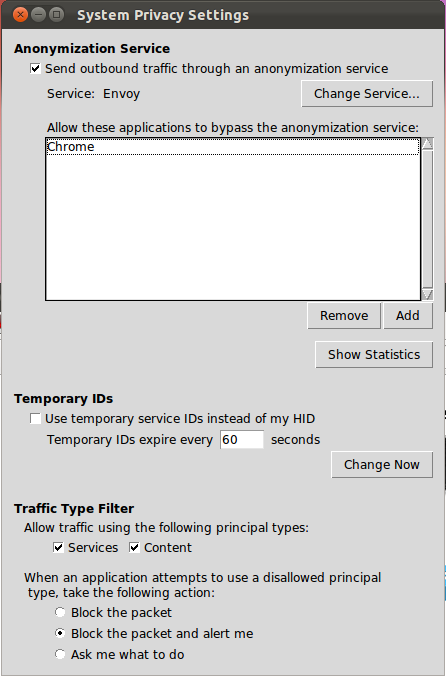
\includegraphics[scale=0.75]{images/privacy-settings.png}
\caption{A preference pane lets the user tell the OS how to anonymize network traffic.}
\label{fig:settings}
\end{figure}

\begin{figure}
\centering
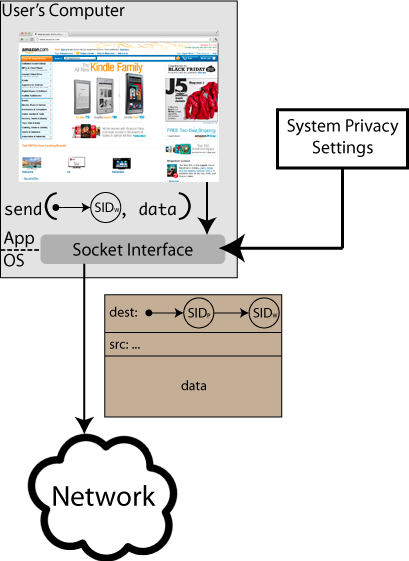
\includegraphics[scale=0.75]{images/socket-control.png}
\caption{System-wide controls affect the behavior of the socket layer, bypassing applications entirely, allowing users to ensure all traffic is sent as per their anonymization settings.}
\label{fig:socket-control}
\end{figure}

But control alone is not enough. Once users have customized the behavior of their systems, they would like a way to verify that their systems are acting on their preferences. To this end, our prototype includes a chart (Figure~\ref{fig:feedback}) which displays to the user counts of three different classes of packets: packets sent through the anonymizer specified in the system preference pane (i.e., packets sent from \texttt{XgetCID()} or from connections established with \texttt{Xconnect()}), packets sent through a different, application-specified anonymizer (\texttt{XgetCIDCustomAnonymizer()} or \texttt{XconnectCustomAnonymizer()}), and packets sent through no anonymizer at all (\texttt{XgetCIDWithoutAnonymizer()} or \texttt{XconnectWithoutAnonymizer()}). Though our interface is simplistic and unpolished, it serves to emphasize the need for system transparency.

\begin{figure}
\centering
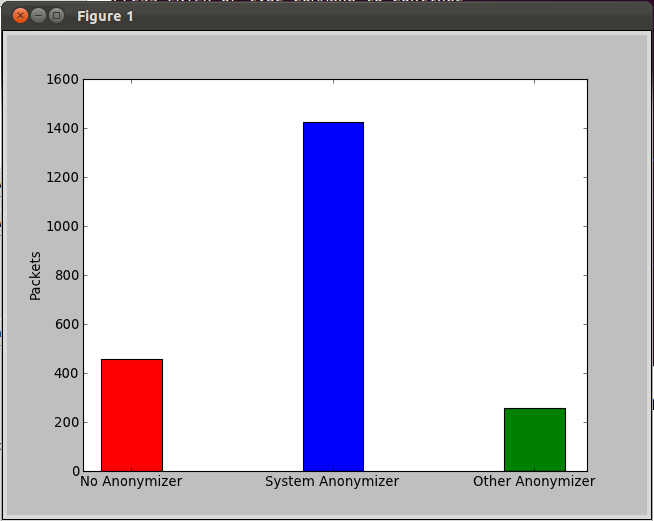
\includegraphics[scale=0.5]{images/feedback.png}
\caption{An example of feedback the operating system might give a user.}
\label{fig:feedback}
\end{figure}


\section{Conclusion}
\label{conclusion}
Anonymity in the Internet is sought by many people for many reasons. We consider the place of anonymity in XIA, with an eye toward verifying that XIA doesn't mix badly with existing approaches and exploring new approaches enabled by XIA. Further, we propose an extension to the XSocket API allowing developers easy access to standard implementations  of these approaches. We also discuss the desirability of an operating system preference pane empowering users to control system-wide traffic anonymity settings.

Our implementation of the extended socket API, the preference pane, and a simple proxy serve to demonstrate the feasibility of proxies as in-network services, act as a basis for future user studies, and uncover new issues relating to anonymity and in-network services in XIA.

\bibliography{FinalWriteup}{}
\bibliographystyle{plain}
\end{document}